% !TEX program = pdflatex
\RequirePackage[l2tabu, orthodox]{nag}
\documentclass{article}

% FONTS
\usepackage[T1]{fontenc}

% Replace default Latin Modern typewriter with its proportional counterpart
% http://www.tug.dk/FontCatalogue/lmoderntypewriterprop/
\renewcommand*\ttdefault{lmvtt}


%%% OPTION 1 - Fourier Math + New Century Schoolbook + ParaType Sans

% % Import Fourier Math (this imposes its own New Century Schoolbook type)
% % http://www.ctan.org/tex-archive/fonts/fouriernc/
%\usepackage{fouriernc}
%\usepackage{amsmath}
% % Replace with TeX Gyre Schola version of New Century Schoolbook (must scale!)
% % http://www.tug.dk/FontCatalogue/tgschola/
%\usepackage[scale=0.92]{tgschola}
%\usepackage[scaled=0.88]{PTSans}

%% OPTION 2 - MathDesign Math + Bitstream Charter + ParaType Sans

% Import MathDesign (this brings along Bitstream Charter)
% http://www.ctan.org/tex-archive/fonts/mathdesign/
\usepackage[bitstream-charter]{mathdesign}
\usepackage{amsmath}
\usepackage[scaled=0.92]{PTSans}


% %%% OPTION 3 - MTPRO 2 Math + Termes Times + ParaType Sans

% \usepackage{tgtermes}
% \usepackage{amsmath}
% \usepackage[subscriptcorrection,
%             amssymbols,
%             mtpbb,
%             mtpcal,
%             nofontinfo  % suppresses all warnings
%            ]{mtpro2}
% \usepackage{scalefnt,letltxmacro}
% \LetLtxMacro{\oldtextsc}{\textsc}
% \renewcommand{\textsc}[1]{\oldtextsc{\scalefont{1.10}#1}}
% \usepackage[scaled=0.92]{PTSans}

% GEOMETRY
\usepackage[
  paper  = letterpaper,
  left   = 1.65in,
  right  = 1.65in,
  top    = 1.0in,
  bottom = 1.0in,
  ]{geometry}

% COLOR
\usepackage[usenames,dvipsnames]{xcolor}
\definecolor{shadecolor}{gray}{0.9}

% SPACING and TEXT
\usepackage[final,expansion=alltext]{microtype}
\usepackage[english]{babel}
\usepackage[parfill]{parskip}
\usepackage{afterpage}
\usepackage{framed}
\usepackage{verbatim}

%redefine the leftbar environment to accept a width and coloring options
\renewenvironment{leftbar}[1][\hsize]
{%
  \def\FrameCommand
  {%
    {\color{Gray}\vrule width 3pt}%
    \hspace{10pt}%
    %\hspace{0pt}\fboxsep=\FrameSep\colorbox{black!10}%
  }%
  \MakeFramed{\hsize#1\advance\hsize-\width\FrameRestore}%
}%
{\endMakeFramed}

% define a paragraph header function
\DeclareRobustCommand{\parhead}[1]{\textbf{#1}~}

% EDITING
% line numbering in left margin
\usepackage{lineno}
\renewcommand\linenumberfont{\normalfont
                             \footnotesize
                             \sffamily
                             \color{SkyBlue}}
% ragged paragraphs in right margin
\usepackage{ragged2e}
\DeclareRobustCommand{\sidenote}[1]{\marginpar{
                                    \RaggedRight
                                    \textcolor{Plum}{\textsf{#1}}}}
% paragraph counter in right margin
\newcommand{\parnum}{\bfseries\P\arabic{parcount}}
\newcounter{parcount}
\newcommand\p{%
    \stepcounter{parcount}%
    \leavevmode\marginpar[\hfill\parnum]{\parnum}%
}
% paragraph helper
%\DeclareRobustCommand{\PP}{\textcolor{Plum}{\P} }

% COUNTERS
\renewcommand{\labelenumi}{\color{black!67}{\arabic{enumi}.}}
\renewcommand{\labelenumii}{{\color{black!67}(\alph{enumii})}}
\renewcommand{\labelitemi}{{\color{black!67}\textbullet}}

% FIGURES
\usepackage{graphicx}
\usepackage[labelfont=bf]{caption}
\usepackage[format=hang]{subcaption}

% TABLES
\usepackage{booktabs}

% ALGORITHMS
\usepackage[algoruled]{algorithm2e}
\usepackage{listings}
\usepackage{fancyvrb}
\fvset{fontsize=\normalsize}

% BIBLIOGRAPHY
\usepackage{natbib}

% HYPERREF
\usepackage[colorlinks,linktoc=all]{hyperref}
\usepackage[all]{hypcap}
\hypersetup{citecolor=BurntOrange}
\hypersetup{linkcolor=MidnightBlue}
\hypersetup{urlcolor=MidnightBlue}

% CLEVEREF must come after HYPERREF
\usepackage[nameinlink]{cleveref}

% ACRONYMS
\usepackage[acronym,smallcaps,nowarn]{glossaries}
% \makeglossaries

% COLOR DEFINITIONS
\newcommand{\red}[1]{\textcolor{BrickRed}{#1}}
\newcommand{\orange}[1]{\textcolor{BurntOrange}{#1}}
\newcommand{\green}[1]{\textcolor{OliveGreen}{#1}}
\newcommand{\blue}[1]{\textcolor{MidnightBlue}{#1}}
\newcommand{\gray}[1]{\textcolor{black!60}{#1}}

% LISTINGS DEFINTIONS
\lstdefinestyle{mystyle}{
    commentstyle=\color{OliveGreen},
    keywordstyle=\color{BurntOrange},
    numberstyle=\tiny\color{black!60},
    stringstyle=\color{MidnightBlue},
    basicstyle=\ttfamily,
    breakatwhitespace=false,
    breaklines=true,
    captionpos=b,
    keepspaces=true,
    numbers=left,
    numbersep=5pt,
    showspaces=false,
    showstringspaces=false,
    showtabs=false,
    tabsize=2
}
\lstset{style=mystyle}

\DeclareRobustCommand{\mb}[1]{\ensuremath{\boldsymbol{\mathbf{#1}}}}
\DeclareRobustCommand{\KL}[2]{\ensuremath{\textrm{KL}\left(#1\;\|\;#2\right)}}

\newcommand{\supp}{\textrm{supp}}

\newcommand{\E}{\mathbb{E}}
\newcommand{\Var}{\mathbb{V}\textrm{ar}}

% Redundant with reals, naturals, below
\newcommand{\bbN}{\mathbb{N}}
\newcommand{\bbZ}{\mathbb{Z}}
\newcommand{\bbR}{\mathbb{R}}
\newcommand{\bbS}{\mathbb{S}}
\newcommand{\bbH}{\mathbb{H}}


\newcommand{\bA}{\boldsymbol{A}}
\newcommand{\bB}{\boldsymbol{B}}
\newcommand{\bC}{\boldsymbol{C}}
\newcommand{\bD}{\boldsymbol{D}}
\newcommand{\bE}{\boldsymbol{E}}
\newcommand{\bF}{\boldsymbol{F}}
\newcommand{\bG}{\boldsymbol{G}}
\newcommand{\bH}{\boldsymbol{H}}
\newcommand{\bI}{\boldsymbol{I}}
\newcommand{\bJ}{\boldsymbol{J}}
\newcommand{\bK}{\boldsymbol{K}}
\newcommand{\bL}{\boldsymbol{L}}
\newcommand{\bM}{\boldsymbol{M}}
\newcommand{\bN}{\boldsymbol{N}}
\newcommand{\bO}{\boldsymbol{O}}
\newcommand{\bP}{\boldsymbol{P}}
\newcommand{\bQ}{\boldsymbol{Q}}
\newcommand{\bR}{\boldsymbol{R}}
\newcommand{\bS}{\boldsymbol{S}}
\newcommand{\bT}{\boldsymbol{T}}
\newcommand{\bU}{\boldsymbol{U}}
\newcommand{\bV}{\boldsymbol{V}}
\newcommand{\bW}{\boldsymbol{W}}
\newcommand{\bX}{\boldsymbol{X}}
\newcommand{\bY}{\boldsymbol{Y}}
\newcommand{\bZ}{\boldsymbol{Z}}
\newcommand{\ba}{\boldsymbol{a}}
\newcommand{\bb}{\boldsymbol{b}}
\newcommand{\bc}{\boldsymbol{c}}
\newcommand{\bd}{\boldsymbol{d}}
\newcommand{\be}{\boldsymbol{e}}
\newcommand{\bbf}{\boldsymbol{f}}
\newcommand{\bg}{\boldsymbol{g}}
\newcommand{\bh}{\boldsymbol{h}}
\newcommand{\bi}{\boldsymbol{i}}
\newcommand{\bj}{\boldsymbol{j}}
\newcommand{\bk}{\boldsymbol{k}}
\newcommand{\bl}{\boldsymbol{l}}
\newcommand{\bbm}{\boldsymbol{m}}
\newcommand{\bn}{\boldsymbol{n}}
\newcommand{\bo}{\boldsymbol{o}}
\newcommand{\bp}{\boldsymbol{p}}
\newcommand{\bq}{\boldsymbol{q}}
\newcommand{\br}{\boldsymbol{r}}
\newcommand{\bs}{\boldsymbol{s}}
\newcommand{\bt}{\boldsymbol{t}}
\newcommand{\bu}{\boldsymbol{u}}
\newcommand{\bv}{\boldsymbol{v}}
\newcommand{\bw}{\boldsymbol{w}}
\newcommand{\bx}{\boldsymbol{x}}
\newcommand{\by}{\boldsymbol{y}}
\newcommand{\bz}{\boldsymbol{z}}

\newcommand{\balpha}{\boldsymbol{\alpha}}
\newcommand{\bbeta}{\boldsymbol{\beta}}
\newcommand{\boldeta}{\boldsymbol{\eta}}
\newcommand{\bkappa}{\boldsymbol{\kappa}}
\newcommand{\bgamma}{\boldsymbol{\gamma}}
\newcommand{\blambda}{\boldsymbol{\lambda}}
\newcommand{\bmu}{\boldsymbol{\mu}}
\newcommand{\bnu}{\boldsymbol{\nu}}
\newcommand{\brho}{\boldsymbol{\rho}}
\newcommand{\bphi}{\boldsymbol{\phi}}
\newcommand{\bpi}{\boldsymbol{\pi}}
\newcommand{\bpsi}{\boldsymbol{\psi}}
\newcommand{\bsigma}{\boldsymbol{\sigma}}
\newcommand{\btheta}{\boldsymbol{\theta}}
\newcommand{\bomega}{\boldsymbol{\omega}}
\newcommand{\bxi}{\boldsymbol{\xi}}
\newcommand{\bGamma}{\boldsymbol{\Gamma}}
\newcommand{\bLambda}{\boldsymbol{\Lambda}}
\newcommand{\bOmega}{\boldsymbol{\Omega}}
\newcommand{\bPhi}{\boldsymbol{\Phi}}
\newcommand{\bPi}{\boldsymbol{\Pi}}
\newcommand{\bPsi}{\boldsymbol{\Psi}}
\newcommand{\bSigma}{\boldsymbol{\Sigma}}
\newcommand{\bTheta}{\boldsymbol{\Theta}}
\newcommand{\bUpsilon}{\boldsymbol{\Upsilon}}
\newcommand{\bXi}{\boldsymbol{\Xi}}
\newcommand{\bepsilon}{\boldsymbol{\epsilon}}

\newcommand{\mcA}{\mathcal{A}}
\newcommand{\mcB}{\mathcal{B}}
\newcommand{\mcC}{\mathcal{C}}
\newcommand{\mcD}{\mathcal{D}}
\newcommand{\mcE}{\mathcal{E}}
\newcommand{\mcF}{\mathcal{F}}
\newcommand{\mcG}{\mathcal{G}}
\newcommand{\mcH}{\mathcal{H}}
\newcommand{\mcI}{\mathcal{I}}
\newcommand{\mcJ}{\mathcal{J}}
\newcommand{\mcK}{\mathcal{K}}
\newcommand{\mcL}{\mathcal{L}}
\newcommand{\mcM}{\mathcal{M}}
\newcommand{\mcN}{\mathcal{N}}
\newcommand{\mcO}{\mathcal{O}}
\newcommand{\mcP}{\mathcal{P}}
\newcommand{\mcQ}{\mathcal{Q}}
\newcommand{\mcR}{\mathcal{R}}
\newcommand{\mcS}{\mathcal{S}}
\newcommand{\mcT}{\mathcal{T}}
\newcommand{\mcU}{\mathcal{U}}
\newcommand{\mcV}{\mathcal{V}}
\newcommand{\mcW}{\mathcal{W}}
\newcommand{\mcX}{\mathcal{X}}
\newcommand{\mcY}{\mathcal{Y}}
\newcommand{\mcZ}{\mathcal{Z}}

\newcommand{\trans}{\mathsf{T}}
\newcommand{\naturals}{\mathbb{N}}
\newcommand{\reals}{\mathbb{R}}
\def\argmax{\operatornamewithlimits{arg\,max}}
\def\argmin{\operatornamewithlimits{arg\,min}}

\newcommand{\distNormal}{\mathcal{N}}
\newcommand{\distGamma}{\mathrm{Gamma}}
\newcommand{\distBernoulli}{\mathrm{Bern}}
\newcommand{\distBinomial}{\mathrm{Bin}}
\newcommand{\distCategorical}{\mathrm{Cat}}
\newcommand{\distDirichlet}{\mathrm{Dir}}
\newcommand{\distMultinomial}{\mathrm{Mult}}
\newcommand{\distPolyaGamma}{\mathrm{PG}}
\newcommand{\distMNIW}{\mathrm{MNIW}}
\newcommand{\distBeta}{\mathrm{Beta}}

\newcommand{\prt}[1]{\frac{\partial}{\partial #1}}
\newcommand{\deriv}[1]{\frac{\mathrm{d}}{\mathrm{d} #1}}


\newcommand{\TODO}[1]{\textcolor{red}{[TODO: #1]}}

\newcommand{\bbI}{\mathbb{I}}
\newcommand{\bbE}{\mathbb{E}}
\newcommand{\bone}{\boldsymbol{1}}
\newcommand{\bigO}{\mathcal{O}}
\newcommand{\iid}[1]{\stackrel{\text{iid}}{#1}}
\newcommand\indep{\protect\mathpalette{\protect\independenT}{\perp}}
\def\independenT#1#2{\mathrel{\rlap{$#1#2$}\mkern4mu{#1#2}}}
\DeclareMathOperator{\Skew}{Skew}
\DeclareMathOperator{\Symm}{Sym}
\DeclareMathOperator{\tr}{tr}

%\DeclareMathOperator{\KL}{KL}
\newcommand{\given}{\, | \,}

\DeclareMathOperator{\diag}{diag}
\let\vec\relax% Set equal to \relax so that LaTeX thinks it's not defined
\DeclareMathOperator{\vec}{vec}
\let\Re\relax
\DeclareMathOperator{\Re}{\textup{Re}}
\let\Im\relax
\DeclareMathOperator{\Im}{\textup{Im}}

% Backcompat: dif and diff both work
\newcommand*\dif{\mathop{}\!\mathrm{d}}
\newcommand*\diff{\mathop{}\!\mathrm{d}}



% \linenumbers

\title{Reparameterizing the Birkhoff Polytope for Variational Permutation Inference}
\author{
  Scott W. Linderman\thanks{These authors contributed equally.}, Gonzalo E. Mena\footnotemark[1], Hal Cooper, \\
  Liam Paninski, and John P. Cunningham\\
  \\
  Columbia University
}

\begin{document}
\maketitle

\begin{abstract}
  How can we efficiently perform posterior inference over the space
  of permutations when there are~$N!$ permutations of a set of~$N$
  elements?  Clearly, estimating a complete probability mass function
  over this space quicky becomes intractable as~$N$ grows. Our goal is
  to derive a tractable algorithm for performing approximate inference
  over this challenging discrete space.  To that end, we consider
  extensions of the recently proposed Gumbel-softmax method, which
  leverages continuous relaxations to perform discrete variational
  inference with reparameterization gradients. While the
  Gumbel-softmax method is not immediately applicable to permutation
  inference, we show that two alternative reparameterizations are both
  comparable to Gumbel-softmax on tractable discrete problems and
  easily extensible to permutation inference. Specifically, we develop
  continuous relaxations of permutation matrices to matrices that are
  either exactly or nearly doubly stochastic, i.e. to points either in
  or near the Birkhoff polytope.  We then derive invertible and
  differentiable maps from densities on unconstrained space to
  densities on or near the Birkhoff polytope. These transformations
  are parameterized by a ``temperature'' that controls how
  concentrated the resulting density is at the extrema of the Birkhoff
  polytope; i.e. at permutation matrices.  This relaxation admits
  variational inference via stochastic gradient ascent over the
  distributions on doubly stochastic matrices (and in the
  zero-temperature limit, on permutation matrices) using Monte Carlo
  estimates of the reparameterized gradient.
\end{abstract}

\section{Introduction}

% Permutation inference central to many machine learning problems
% - Matching problems
% - Multiple object tracking
% - Ranking
% - As latent step in a generative model
Permutation inference is central to many modern machine learning
problems.  Identity management~\citep{guibas2008identity} and
multiple-object tracking~\citep{shin2005lazy, kondor2007multi} are
fundamentally concerned with finding a permutation that maps an
observed set of items to a set of canonical labels.
Ranking problems, critical to search and recommender systems, require
inference over the space of item orderings \citep{meilua2007consensus,
  lebanon2008non, adams2011ranking}.  Moreover, many probabilistic models, like
preferential attachment network models~\citep{bloem2016random} and
repulsive point process models~\citep{rao2016bayesian}, incorporate a
latent permutation into their generative processes; inference over
model parameters requires integrating over the set of permutations
that could have given rise to the observed data.  In many of these
settings, permutation inference is but one component of a larger
estimation problem involving unknown model parameters and hierarchical
structure.

% Emphasize the importance of Bayesian approach and recent advances
% in variational inference
The task of computing optimal point estimates of permutations under
various loss functions has been well studied
in the combinatorial optimization literature ~\citep{kuhn1955hungarian, munkres1957algorithms,
  lawler1963quadratic}. However, many probabilistic tasks require reasoning
about uncertainty regarding permutation matrices.  A variety of
Bayesian permutation inference algorithms have been proposed, leveraging
Markov chain Monte Carlo methods \citep{diaconis1988group}, Fourier
representations~\citep{kondor2007multi, huang2009fourier}, as well as
convex~\citep{lim2014beyond} and
continuous~\citep{plis2011directional} relaxations for approximating
the posterior distribution.  Given recent advances in scaling
variational Bayesian inference, largely driven by efficient Monte
Carlo estimators of gradients of the variational lower bound
\citep{Kingma2014, rezende2014stochastic}, we revisit the problem of
permutation inference from a variational perspective.

% Gumbel-softmax motivation
Continuous relaxations underlie many approximate algorithms for
discrete optimization and inference.  After relaxation, we can
capitalize on local gradients and curvature information. Indeed, this
is the motivation for the recently proposed Gumbel-softmax method for
discrete variational inference~\citep{jang2016categorical,
  maddison2016concrete}.  It is based on the following observation:
categorical distributions may be viewed as atomic densities
on the vertices of the simplex; by relaxing this to a continuous
density on the interior of the simplex we can approximate the discrete
inference problem with a continuous one and thereby capitalize on
reparameterization gradients~\citep{Kingma2014, rezende2014stochastic}
to optimize a variational lower bound on the marginal likelihood.
Critically, the Gumbel-softmax method has a temperature parameter that
tunes the degree to which the continuous density concentrates around
the vertices, and recovers truly discrete inference in the
zero-temperature limit.

% Discrete/Simplex <-> Permutation/Birkhoff analogy 
Just as one-hot vectors (discrete random variables) are the vertices
of the simplex, permutation matrices are the vertices of the Birkhoff
polytope, i.e. the set of doubly stochastic matrices.  Thus, we seek
temperature-controlled relaxations of atomic densities on permutation
matrices to continuous densities on the interior of the Birkhoff
polytope.  Unfortunately, the dual constraints of row- and
column-normalization required of doubly stochastic matrices present
difficulties that are not faced in the categorical setting. However,
we derive a variety of alternative continuous relaxations for the
simplex and show that: (i) these relaxations achieve comparable
performance to the Gumbel-softmax on tractable discrete inference
tasks; and (ii) they naturally extend to relaxations of permutation
inference problems.

% Paper structure
The remainder of this paper is structured as follows:
Section~\ref{sec:relatedwork} discusses related work on Bayesian
permutation inference and the continuous relaxations for discrete
inference, including the Gumbel-softmax method.
Section~\ref{sec:alternative} introduces alternative relaxations for
discrete variational inference, and Section~\ref{sec:permutation}
presents our primary contribution: a set of relaxations for
permutation matrices. Section~\ref{sec:results} presents a variety of
experiments that illustrate the benefits of the proposed variational
approach.
  
\section{Related Work}
\label{sec:relatedwork}

\parhead{Bayesian permutation inference. } As mentioned above, a
number of previous works have considered approximate methods of
posterior inference over the space of permutations. When a point
estimate will suffice, convex relations are commonly employed~\citep{fogel2013convex,
  lim2014beyond}. Given noisy measurements of a sum of a small number of
permutation matrices, we can recover the underlying coefficients
via a convex optimization penalized by the norm induced by the Birkhoff
polytope~\citep{chandrasekaran2012convex}.  For some ranking problems,
we can rewrite the objective function in terms of the expected 
assignment probabilities under a distribution over permutation matrices, which
in turn are points in the Birkhoff polytope. \citet{adams2011ranking}
leveraged this property to develop stochastic gradient descent algorithms
that minimize these objective functions, using Sinkhorn propagation~\citep{knight2008sinkhorn}
as a differentiable map from the positive orthant to the Birkhoff polytope.
We will use the same approach in one of our proposed methods. 


When a point estimate is insufficient, it may be possible to turn
efficient algorithms for optimizing linear cost functions over the set
of permutation matrices into efficient sampling algorithms using
Perturb-and-MAP \citep{li2013efficient}.  For simple problems, Markov
chain Monte Carlo (MCMC) algorithms can perform quite well by simply
using Metropolis-Hastings proposals to swap assignments at random
\citep{diaconis1988group}.  Such methods ultimately rely on a random
walk to explore the high dimensional space of permutations.
\citet{harrison2013importance} developed an importance sampling
algorithm that fills in count matrices one row at a time, leveraging
column- and row-sum constraints, and showed promising results for
matrices with~$O(100)$ rows and columns.  Another line of work
considers inference in the spectral domain, approximating
distributions over permutations with the low frequency Fourier
components~\citep{kondor2007multi, huang2009fourier}.  Perhaps most
relevant to this work, \citet{plis2011directional} propose a
continuous relaxation from permutation matrices to points on a
hypersphere, and then use the von Mises-Fisher (vMF) distribution to
model distributions on the sphere's surface. While the vMF
distribution does have a concentration parameter, as the concentration
goes to infinity, the distribution converges to a point on the sphere.
By contrast, we will derive temperature-controlled densities over
points inside or near the Birkhoff polytope such that as the temperature
goes to zero, the distribution converges to an atomic density on
permutation matrices.

\parhead{Variational inference and the reparameterization trick.}
Variational Bayesian inference algorithms aim to approximate the
posterior distribution~$p(x \given y)$ with a more tractable
distribution~$q(x; \theta)$, where ``tractable'' means that, at a
minimum, we can sample~$q$ and evaluate it pointwise (including
its normalization constant).  We find this approximate distribution
by searching for the parameters~$\theta$ that minimize the Kullback-Leibler (KL)
divergence between~$q$ and the true posterior, or equivalently,
maximize the evidence lower bound (ELBO),
\begin{align}
  \mcL(\theta) &\triangleq \bbE_q \left[ \log p(x, y) - \log q(x; \theta) \right].
\end{align}
Perhaps the simplest method of optimizing the ELBO is stochastic
gradient ascent. 
However, computing~$\nabla_\theta \mcL(\theta)$ requires some care
since the ELBO contains an expectation with respect to a distribution
that depends on these parameters.

When~$x$ is a continuous random variable, we can often go one step
further and leverage the ``reparameterization trick''
\citep{Salimans2013, Kingma2014}.  Specifically, in some cases we can
simulate from~$q$ via the following equivalence,
\begin{align}
  \label{eq:reparam}
  x &\sim q(x; \theta)
      & \iff & &  
  \xi &\sim r(\xi), \quad x = g(\theta, \xi),
\end{align}
where~$r$ is a distribution on the ``noise''~$\xi$ and
where~$g(\theta, \xi)$ is a deterministic and differentiable
function. For example,
if~${q(x; \theta) = \distNormal(x \given \theta, 1)}$, we can
reparameterize by setting the noise distribution
to~${r(\xi) = \distNormal(\xi \given 0, 1)}$ and using the
transformation~${g(\theta, \xi) = \theta + \xi}$.  The
reparameterization trick effectively ``factors out'' the randomness
of~$q$. With this transformation, we can bring the gradient inside the
expectation as follows,
\begin{align}
  \nabla_\theta \mcL(\theta) 
  &= \E_{r(\xi)} \left[ \nabla_\theta \log p(g(\theta, \xi) \given y)
    - \nabla_\theta  \log q(g(\theta, \xi); \theta) \right].
\end{align}
This gradient can be estimated with Monte Carlo, and, in practice,
this leads to lower variance estimates of the gradient than, for
example, the score function estimator \citep{Williams1992, Glynn1990}.
However, for $g$ to be differentiable $x$ needs to be continuous.

\begin{figure*}[t]
  \centering
  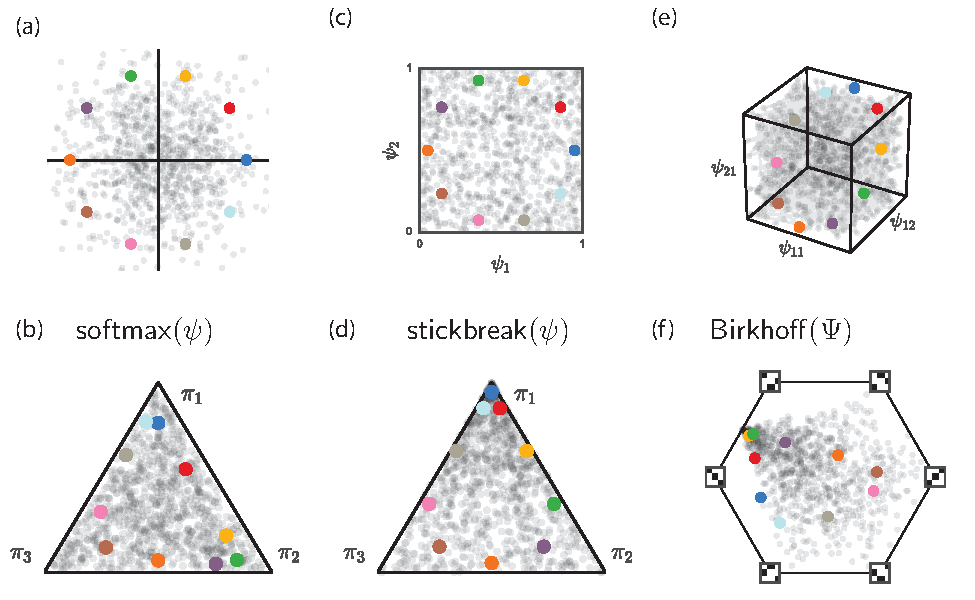
\includegraphics[width=5.in]{../figures/figure1.pdf} 
  \caption{Reparameterizations of discrete polytopes.  (a,b) The
    Gumbel-softmax, or ``Concrete'' transformation maps points
    ${\psi \in \reals^N}$ to points~${x \in \Delta_{N}}$ by adding
    noise and applying the softmax.  Here we show a slice for~$N=3$
    with~$\psi_3=0$. Colored points are aids to visualize the
    transformation.  (c,d) Stick-breaking offers and alternative
    transformation, here from points~$\psi \in [0,1]^{N-1}$ to~$\Delta_N$.
    The ordering of the stick-breaking induces an asymmetry in the
    transformation.  (e,f) We extend this stick-breaking transformation
    to reparameterize the Birkhoff polytope, i.e. the set of doubly
    stochastic matrices. Here,~$\mcB_3$ is reparameterized in terms
    of matrices~$\Psi \in [0,1]^{2 \times 2}$, of which three coordinates
    are shown in (e).  These points are mapped to doubly stochastic
    matrices, which we have projected onto~$\reals^2$ in panel~(f).}
\label{fig:transforms}
\end{figure*}

\parhead{Continuous relaxations for discrete variational inference.}
Recently, there have been a number of proposals for extending the
reparameterization trick to high dimensional discrete
problems\footnote{Discrete inference is only problematic in the high
  dimensional case, since in low dimensional problems we can enumerate
  the possible values of~$x$ and compute the normalizing
  constant~$p(y) = \sum_x p(y, x)$.} by relaxing them to analogous
continuous problems \citep{maddison2016concrete, jang2016categorical,
  kusner2016gans}.  These approaches are based on the following
observation: one-hot vectors~$x \in \{0,1\}^N$ can alternatively be
viewed as vertices of the simplex~$\Delta_N$; likewise, discrete
probability mass functions~$q(x; \theta)$ can be seen as atomic
densities on the vertices of the simplex.  This motivates a natural
relaxation: let~$x$ assume any value in the simplex, not just the
vertices, and let~$q(x; \theta)$ be a density on the interior of the
simplex.  One way to define such a density is via the following
reparameterization,
\begin{align}
  \xi &\sim r(\xi), \\
  g(\theta, \xi) &= \left[ \frac{\theta_1 + \xi_1}{\sum_{n=1}^N \theta_n + \xi_n},
      \ldots,
      \frac{\theta_N + \xi_N}{\sum_{n=1}^N \theta_n + \xi_n}
      \right]
    \triangleq \mathrm{softmax}(\theta + \xi),
\end{align}
where~${\xi, \theta \in \reals^N}$.  

In the aforementioned papers, the noise is assumed to be a vector of
independent Gumbel random variables,
i.e.~${p(\xi) = \prod_{n=1}^N \mathrm{Gumbel}(\xi_n \given 0, 1)}$.
This choice leads to a nicely interpretable model: adding Gumbel noise
and taking the \emph{argmax} of~$\theta + \xi$ yields an exact sample from~$\pi = \mathrm{softmax}(\theta)$, thus
the \emph{softmax} of~$\theta + \xi$ is a natural relaxation. Ultimately,
however, this is just a continuous relaxation of an atomic density to
a continuous density.

\section{Alternative relaxations for categorical random variables}
\label{sec:alternative}
Here we introduce two alternative ways of conceiving a relaxed version
of a discrete random variable, both of which are amenable to the
reparameterization trick. However, unlike the Gumbel-Softmax, these
relaxations enable extensions to more complex combinatorial objects
like permutations.

\subsection{Stick-breaking transformations}
First, let us consider an alternative reparameterization of the simplex
via a stick breaking construction. We break this into two steps. First,
we transform the noise and parameters to a point in the~${N-1}$ dimensional
unit hypercube,
\begin{align}
  \xi &\sim r(\xi), & 
  \psi & = f(\theta, \xi),
\end{align}
where~${\psi \in [0,1]^{N-1}}$. Then we transform the hypercube to~$\Delta_N$
  via a stick-breaking transformation,
\begin{align}
  x_n = g_n(\psi)
  &= \begin{cases}
    \psi_1 & n=1, \\
    \psi_n \left(1- \sum_{m=1}^{n-1} x_m \right) & 1 < n < N, \\
    1- \sum_{n=1}^{N-1} x_n & n=N.
    \end{cases}
\end{align}
The intermediate values~$\psi_n$ can seen as the fraction of the
remaining ``stick'' of probability mass assigned to~${\pi}_n$.  In
addition to its use in Bayesian nonparametrics, this type of
transformation has been used in efficient MCMC algorithms for
multinomial and categorical inference \citep{linderman2015dependent}.

We focus on standard Gaussian noise~${r(\xi) = \distNormal(0,I)}$
and we take~$f$ to be a logistic
transformation~${\psi_n = \sigma((\mu_n + \eta_n \xi_n) / \tau)}$,
where ${\sigma(u) = (1+e^{-u})^{-1}}$ is the logistic function
and~$\tau$ is a \emph{temperature} parameter.  This
\emph{logistic-normal stick breaking} transformation is parameterized
by~${\theta = \{\mu_n, \eta_n\}_{n=1}^{N-1}}$, and it enjoys following
properties: i)~the density of~$x$ can be expressed in closed form as a
function of~$\mu_n$ and~$\eta_n^2$; ii)~the temperature~$\tau$
controls how concentrated $p(x)$ is at the vertices of the simplex;
iii)~with appropriate choices of parameters, in the limit
~$\tau \to 0$ we can recover any categorial distribution, i.e., the
density becomes concentrated on atoms at the~$N$ vertices; and iv)~as
~$\tau \to \infty$, the density concentrates on a point in the
interior of the simplex determined by the parameters. For all
intermediate temperatures, the density is continuous on the simplex.

Note that the logistic-normal stick breaking transformation one of
many available. For example, we could take~$r$ and $f$ to be a
reparameterization of the Kumaraswamy of beta distributions on the
unit interval. The former is easily reparameterizable and the
latter---which leads to the generalized Dirichlet distribution on the
simplex---can be reparameterized following~\citet{naesseth2017reparameterization}. We include proofs of points (i-iv) and details of the Kumaraswamy and beta stick breaking constructions in the appendix.

\subsection{Rounding transformations}
Both the Gumbel-softmax and stick-breaking relaxations consider
distributions on the simplex, and while this
offers an intuitive interpretation, it is not strictly required.  For
example, first consider a distribution on~$\psi \in \reals^N$. These
points are the rounded to the nearest vertex of the simplex via the
operator,
\begin{align}
  \mathrm{round}(\psi) &= \argmin_{e_n} \| \psi - e_n \|.
\end{align}
% This operator partitions~$\reals^N$ into ``Voronoi'' cells
% centered on the~$N$ vertices,
% \begin{align}
%   V_n &=
%         \left\{\psi \in \reals^N: \, 
%         \| \psi - e_n \| \leq \| \psi - e_m \| \;
%         \forall m \in 1, \ldots, N \right\}.
% \end{align}
Unfortunately this rounding operator is non-invertible and
non-differentiable.  Thus, we instead consider a map that pulls a
point towards its rounded value, by taking a convex combination
between both. Specifically, we consider the following reparameterization:
\begin{align}
  \xi &\sim p(\xi), \\
  \psi &= f(\theta, \xi), \\
  x &=  \tau \psi + (1-\tau) \cdot \mathrm{round}(\psi) .
\end{align}
In the zero-temperature limit we recover a discrete distribution on
the vertices. For~$\tau > 0$, the distribution is continuous
on~$\reals^N$. If the distribution of~$\psi$ is concentrated
near the simplex---e.g. if~$\theta$ is a point on the simplex
and~$\xi$ is small, additive Gaussian noise---the rounded points
will lie close to the simplex as well. Moreover, this technique
is easily generalized to more complex discrete polytopes. 
% Moreover, this approach can be generalized to arbitrary discrete we
% can represent any arbitrary categorical distribution over one-hot
% vectors. This is shown in the appendix.
 
\section{Continuous relaxations of permutation distributions}
\label{sec:permutation}

Just as one-hot vectors are the vertices of the simplex, the
Birkhoff-von Neumann theorem states that permutation matrices~$X$ are
vertices of the convex hull of doubly stochastic matrices. By analogy,
it is natural to relax to~${X \in \mcB_N \subset [0,1]^{N \times N}}$,
the Birkhoff polytope of doubly stochastic matrices defined by,
\begin{align}
  \mcB_N &= \left \{X: \;
           x_{m,n} \geq 0 \, \forall m,n \in [N]; \;
           \sum_{n=1}^N x_{m,n} = 1 \, \forall m \in [N]; \;
           \sum_{m=1}^N x_{m,n} =1 \, \forall n \in [N]\right\}.
\end{align}
Due to these linear row- and column-normalization
constraints,~$\mcB_N$ lies within a~${(N-1)^2}$ dimensional subspace.
Unfortunately, these constraints also present difficulties to
reparameterization.  Next we show how the stick-breaking and rounding
reparameterizations can be extended to the Birkhoff polytope.

\subsection{Stick-breaking transformations of the Birkhoff polytope}
We now derive an invertible and differentiable
transformation,~$g: \reals^{(N-1) \times (N-1)} \to \mcB_n$ by
extending the original stick-breaking transformation with minor
modifications to accomodate the additional constraints of doubly
stochastic matrices. This can be used to define a density
on~$\mcB_N$. Let~$\Psi$ be an matrix
in~${[0,1]^{(N-1) \times (N-1)}}$; we will transform it into a doubly
stochastic matrix,~$X \in [0,1]^{N \times N}$ by working entry by
entry, starting in the top left and raster scanning left to right then
top to bottom. Denote the~$(m,n)$-th entries of~$\Psi$ and~$X$
by~$\psi_{mn}$ and~${x}_{mn}$, respectively.

The first entry is given by, $x_{11} = \psi_{11}$.  As we work left to
right in the first row, the ``remaining stick'' length decreases as we
add new entries. This reflects the row normalization constraints.
Thus,
\begin{align}
  x_{1n} &= \psi_{1n} \left(1 - \sum_{k=1}^{n-1} x_{1k} \right)  & &  \text{for } n=2, \ldots, N-1\\
  x_{1N} &= 1 - \sum_{n=1}^{N-1} x_{1n}
\end{align}
So far, this is exactly as in the stick breaking construction
above. However, the remaining rows must now conform to both row- and
column-constraints. That is,
\begin{align}
x_{mn} &\leq 1- \sum_{k=1}^{n-1} x_{mk} & & \text{(row sum)} \\
x_{mn} &\leq 1- \sum_{k=1}^{m-1} x_{kn} & & \text{(column sum)}.
\end{align}
Moreover, there is also a lower bound on~$x_{mn}$. This entry must
claim enough of the stick such that what is leftover ``fits'' within
the confines imposed by subsequent column sums. That is, each column
sum places an upper bound on the amount that may be attributed to any
subsequent entry. If the remaining stick exceeds the sum of these
upper bounds, the matrix will not be doubly stochastic.  Thus,
\begin{align}
\underbrace{1 - \sum_{k=1}^n x_{mk}}_{\text{remaining stick}}
  &\leq \underbrace{\sum_{j=n+1}^N (1- \sum_{k=1}^{m-1} x_{kj})}_{
    \text{remaining upper bounds}}.
\end{align}
Rearranging terms, we have,
\begin{align}
x_{mn} &\geq 1- \sum_{k=1}^{n-1} x_{mk} - \sum_{j=n+1}^N (1- \sum_{k=1}^{m-1} x_{kj}) \\
&= 1 - N + n - \sum_{k=1}^{n-1} x_{mk}  +  \sum_{k=1}^{m-1} \sum_{j=n+1}^N x_{kj}
\end{align}
Of course, this bound is only relevant if the right hand side is greater than zero.
Taken together,~$x_{mn}$ is bounded by,
\begin{align}
\ell_{mn} &\leq x_{mn} \leq u_{mn} \\
\ell_{mn} &\triangleq \max \left \{0, \, 1 - N + n - \sum_{k=1}^{n-1} x_{mk}  +  \sum_{k=1}^{m-1} \sum_{j=n+1}^N x_{kj} \right \}
\\
u_{mn} &\triangleq 
\min \left \{1- \sum_{k=1}^{n-1} x_{mk}, \,
1- \sum_{k=1}^{m-1} x_{kn} \right\}.
\end{align}
Thus, we define,
\begin{align}
  x_{mn} &= \ell_{mn} + (\psi_{mn} (u_{mn} - \ell_{mn}).
\end{align}

The inverse transformation from~$X$ to $\Psi$ is analogous.
We start by computing~$\psi_{11}$ and then progressively compute
upper and lower bounds and set,
\begin{align}
\psi_{mn} &= \frac{x_{mn} - \ell_{mn}}{u_{mn} - \ell_{mn}}.
\end{align}


\subsection{Rounding toward permutation matrices}

The rounding-based relaxation immediately extends to the permutation
case.  Now we simulate matrices~$\Psi \in \reals^{N \times N}$ and
round them to the nearest permutation matrix by solving a matching
problem.  This can be done in $O(N^3)$ time with the Hungarian
algorithm~\citep{kuhn1955hungarian, munkres1957algorithms}.  As
before, if~$\Psi$ is close to the Birkhoff polytope, its rounded
value~$X$ will be as well.  Fortunately, it is easy to generate a
distribution that concentrates near~$\mcB_N$.  We use the
reparameterization~${\Psi = \widetilde{\Theta} + \Xi}$,
where~${r(\vec(\Xi)) = \distNormal(0, I)}$, and then we
define~${\widetilde{\Theta}}$ to be the
result of applying a fixed number of Sinkhorn propagation~\citep{knight2008sinkhorn} steps
to the unconstrained matrix~$\Theta \in \reals^{N \times N}$.
Since the Sinkhorn algorithm is differentiable, we can backpropagate
gradients through this procedure~\citep[c.f.][]{adams2011ranking}.
Note that even though Sinkhorn is non-invertible, we can still
evaluate the density of~$q(X; \theta)$ since it applies \emph{before}
the introduction of the random noise~$\Xi$. 


\section{Results}
\label{sec:results}

We are interested in two principal questions: (i) how sensitive
are categorical relaxations to the choice of Gumbel-softmax,
stick-breaking, or categorical reparameterization? (ii) how
well can the stick-breaking and rounding reparameterizations
of the Birkhoff polytope approximate the true posterior distribution
over permutations in tractable, low-dimensional cases? and (iii)
when, if ever, do our proposed continuous relaxations offer
advantages over alternative approximate Bayesian permutation
inference algorithms?  We will address these questions in turn,
but first we discuss some practical details of our experimental
protocol.

\subsection{Experimental protocol}
\parhead{Continuous prior distributions. } Continuous relaxations requires
re-thinking of the objective. As in \cite{maddison2016concrete}, we
maximize a relaxed ELBO, for which we need to specify a new continuous
prior $p(x)$ over the latent variables.
% Not sure I agree with all of this...
% This prior should be peaked around
% the discrete points for which inference is required, so we can
% conceive the original discrete ELBO through a limiting process. Good,
% peaked priors are necessary as the likelihood $p(y \given x)$ could be
% large for points that have nothing to do with the original problem,
% leading to nonsensical solutions. There is a trade-off, though: priors
% that are too peaked will lead to multiple local maxima of the ELBO,
% preventing optimizers from achieving the right solution. Then, for
% optimal performance the prior has to be treated as a
% hyperparameter.
For the categorical experiments, we use a mixture of Gaussians around
each vertex,~${p(x) = \tfrac{1}{N} \sum_{n=1}^N \distNormal(x \given e_k, \eta^2)}$. For permutations, we use a mixture of Gaussians for each
dimension,
\begin{align}
  p(X) &= \prod_{m=1}^N \prod_{n=1}^N
  \frac{1}{2} \left(\distNormal(x_{mn} \given 0, \eta^2) + \distNormal(x_{mn} \given 1, \eta^2 \right).
  \end{align}
Although this prior puts significant mass invalid points
(e.g.~$\bone$), it penalizes $X$ that far from~$\mcB_N$.

\parhead{Estimating the ELBO. } Notice in all the relaxations
discussed here,~${x = g(\psi)}$ and~${\psi = f(\theta,
  \xi)}$. Moreover, both~$g$ and~$f$ are differentiable and invertible
functions. Therefore, by the change of variable theorem and the law of
the unconscious statistician:
\begin{align}
  \bbE_{r(\xi)} \left[- \log q(g(f(\theta, \xi)); \theta) \right]
  &= \bbH(\psi; \theta)+
    \bbE_{r(\xi)}\left[\log \left|\frac{\partial}{\partial \psi} g(f(\theta, \xi)) \right| \right],
  \end{align}
where~$\bbH$ is the entropy and the term inside of the expectation
is the (log Jacobian of $g$ evaluated at $\psi =
f(\theta,\xi)$. Then, if this Jacobian and the entropy of $\psi$ are
available we can consider an unbiased, Monte Carlo estimator for the ELBO.
% \begin{align}
%   \hat{\mcL}(\theta) = Entropy(\psi) +  \frac{1}{L}\sum_{l=1}^L \left[ \log p(y,  g(\theta, \xi_l) ) +  \log |DF(g(\theta, \xi_l)|\right].
% \end{align}
For example, in the rounding transformation, $g$ is piecewise linear
\footnote{The set of discontinuities has Lebesgue measure zero so we
  can still apply the change of variables theorem.} and
$\log | \tfrac{\partial}{\partial \psi} g(f(\theta, \xi)) |= N\log
\tau$. Also, if $\psi$ is Gaussian its entropy is given by
$N\log(\eta^2 2\pi e )/2$.


\subsection{Variational Autoencoders (VAE) with categorical latent variables}
We first demonstrate that our proposed relaxations are sensible for
categorical random variables. We considered the density estimation
task on MNIST digits, as in \cite{maddison2016concrete,
  jang2016categorical}, where observed digits are reconstructed from a
latent discrete code. We used the continuous ELBO for training, and
evaluated performance based on the marginal likelihood, estimated
through the multi-sample variational objective of the discretized
model (via rounding the samples $\pi$) with $m=1000$. We trained our
models using ADAM in Tensorflow and compared agains the method of
\cite{jang2016categorical}, finding similar results (Table 1). Our
best results were obtained with rounding. Our results suggest our
methods provide a viable alternative to the Gumbel-Softmax. Figure
\ref{fig:VAE} shows a random selection of reconstructed images using
the different approaches.  By eye, the reconstructed images
and the latent codes seem very comparable. 


\begin{table}[t]
  \caption{Summary of results in VAE}
  \label{sample-table}
  \centering
  \begin{tabular}{llll}

    %\multicolumn{4}{Method}                   \\
    \given rule

    & Gumbel-Softmax    & Rounding & Stick-breaking\\
    \cmidrule{2-4}
    - $\log p(x)$ & 113.9  & $\sim$106.9  & 12    \\
        \bottomrule
  \end{tabular}
\end{table}


 \subsection{Synthetic matching experiments}
 To assess the quality of our approximations for distributions over
 permutations, we considered a toy matching problem in which we are given the locations of~$N$ cluster centers and a corresponding set of~$N$
 observations, one for each cluster, corrupted by Gaussian noise.
 Moreover, the observations are permuted so there is no correspondence
 between the order of observations and the order of the cluster centers.
 The goal is to recover the posterior distribution over permutations.
 For~$N=6$, we can explicitly enumerate the~$N!=720$ permutations and
 compute the posterior exactly. 

 We measured the discrepancy using the Battacharya distance (BD)
 between true posterior and an empirical estimate of the inferred
 posterior constructed by sampling from $q(X; \theta)$ and 'rounding'
 to the nearest permutation using the Hungarian algorithm. We found
 that our methods provide reasonable approximations to the true
 posterior, allowing us to represent more complex distributions over
 permutations than, e.g., simple Mallows distribution around the MAP
 estimate. Figure \ref{fig:synthetic} shows
 examples of true posteriors (ranked) and their approximations, and
 quantifies the discrepancies by the distribution of the BD.

 \begin{figure*}[t] 
   \centering
   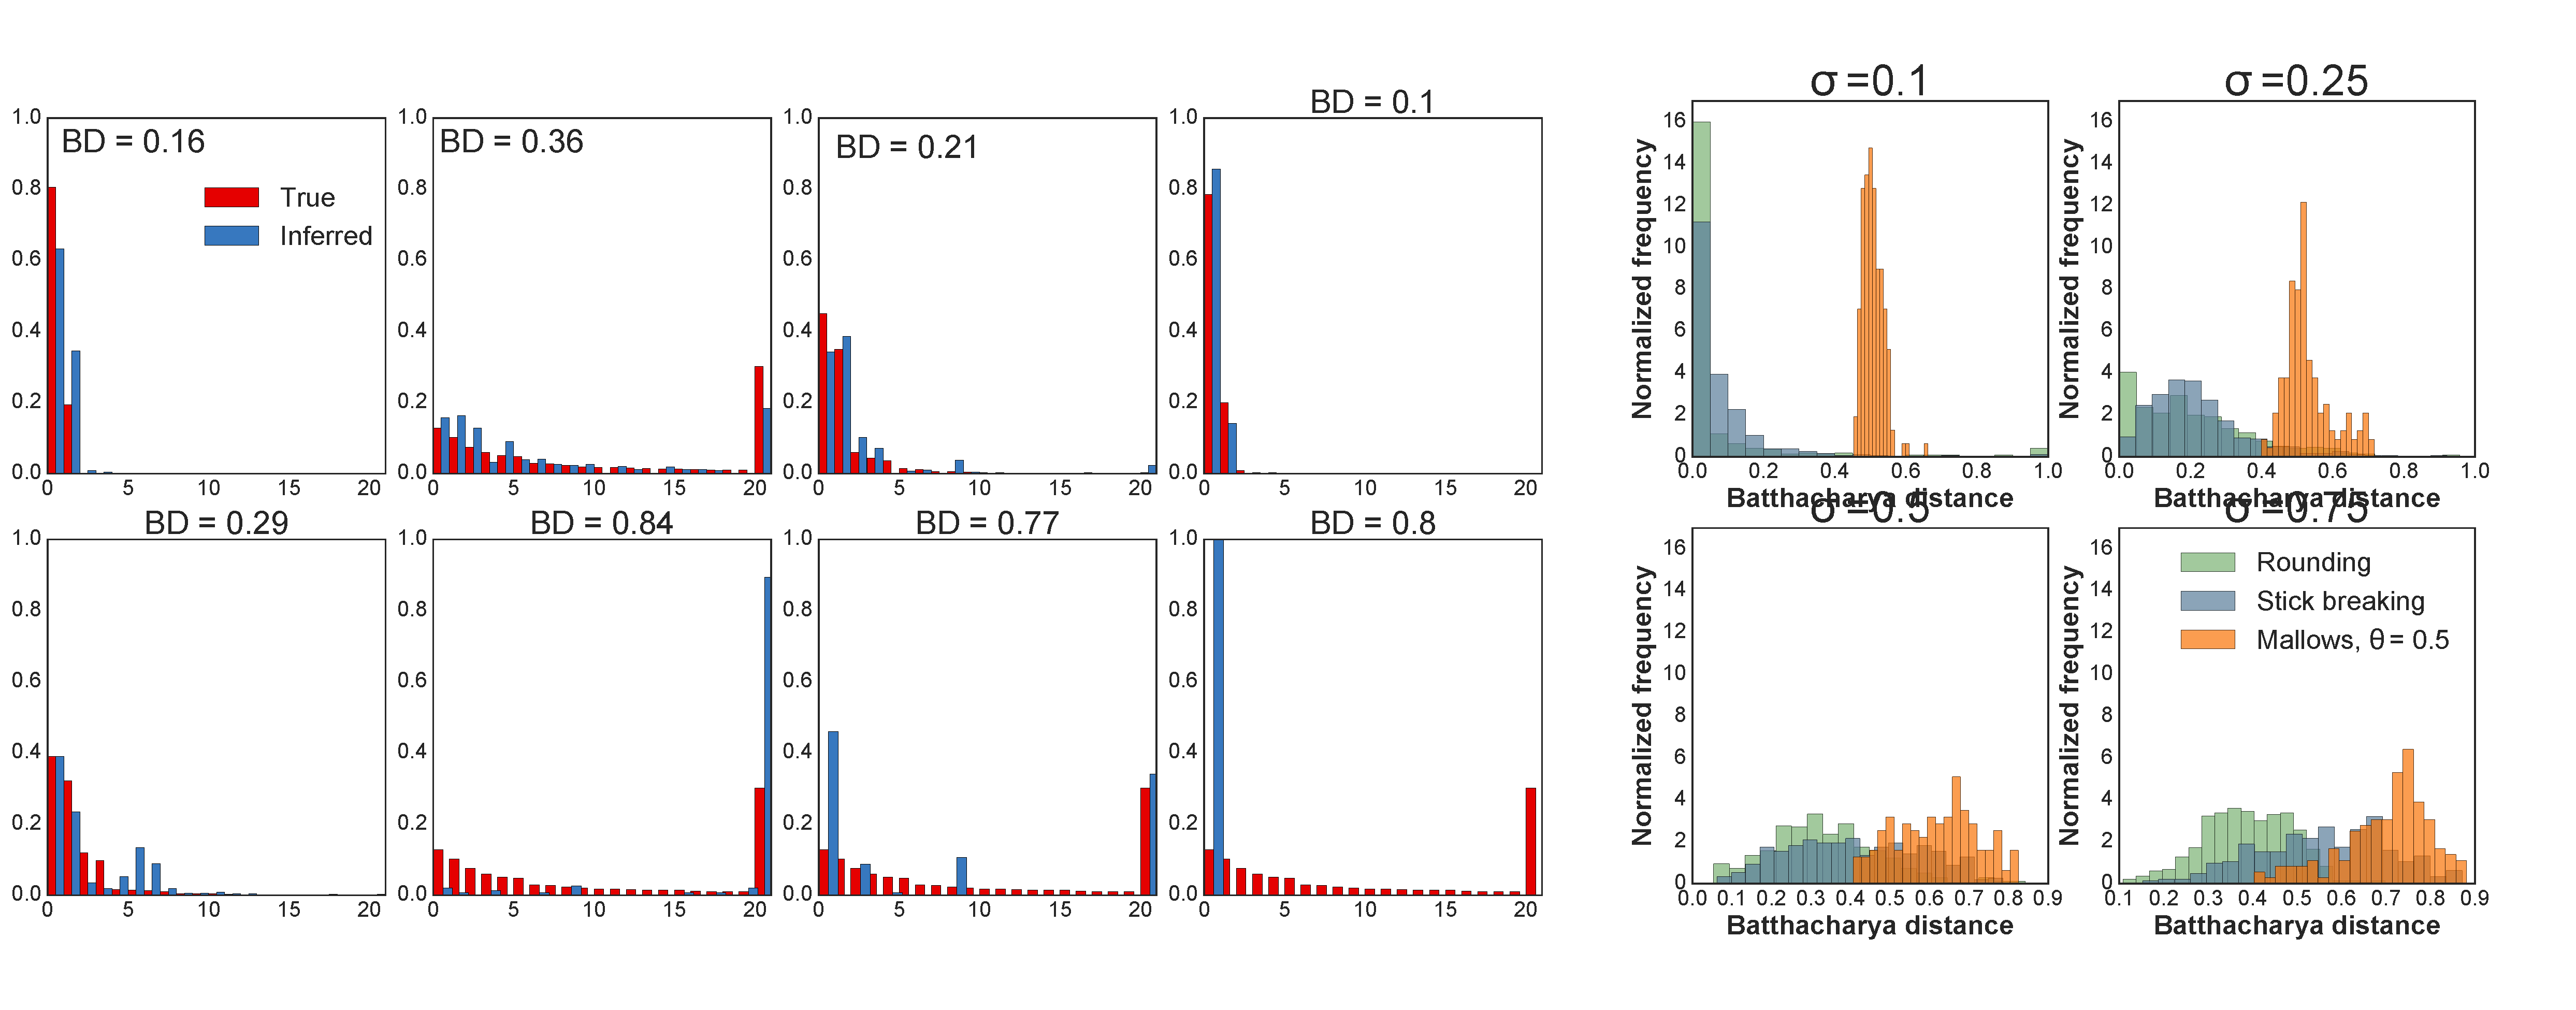
\includegraphics[width=1.0\textwidth]{../figures/figure5.pdf}
   \caption{Left: Side-by-side bar plots of the true and inferred
     posterior distributions along the corresponding Bhattacharya distance.
     Right: comparison of Bhattacharya distance between true and inferred
   posterior using the rounding transformation, the stick breaking transformation, and the Mallows distribution.  Histograms are derived from HOW MANY randomly generated matching problems.  }
\label{fig:VAE}
\end{figure*}

\label{sec:synthetic}


\begin{figure*}[t]
  \centering
  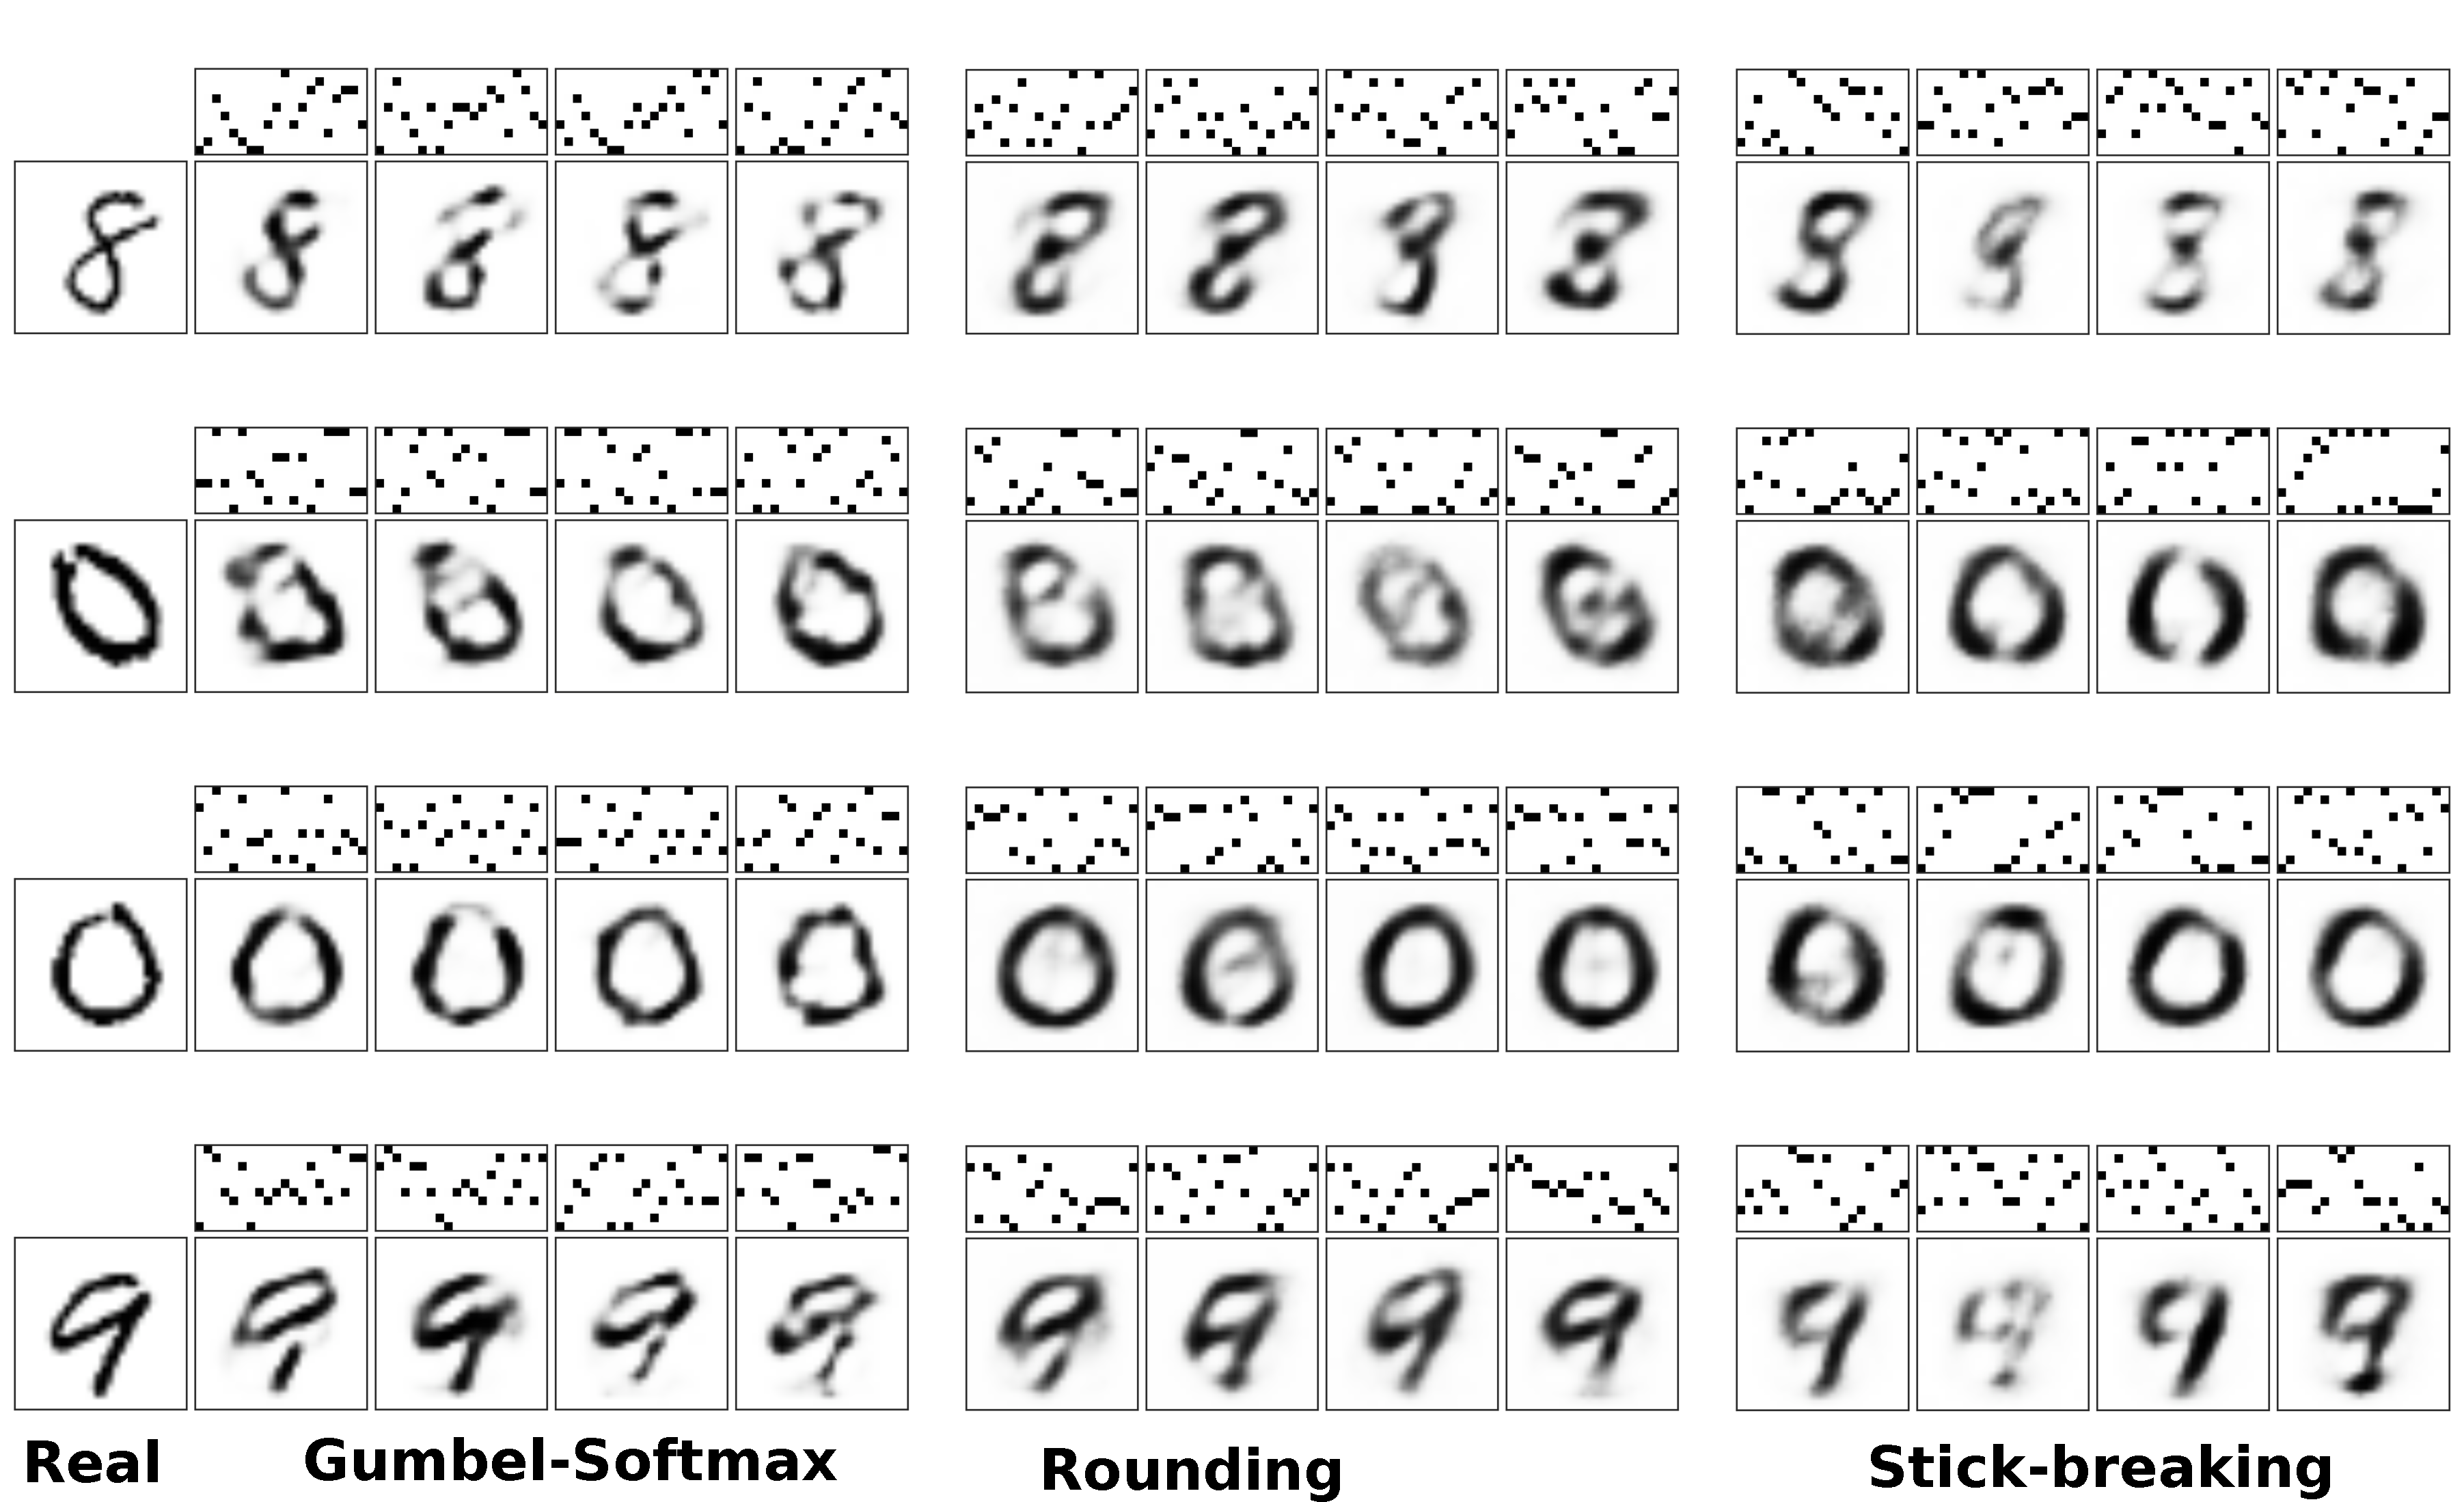
\includegraphics[width=5.in]{../figures/figure4.pdf} 
  \caption{Examples of true and reconstructed digits from their corresponding random codes using with $N=20$ categorical variables with $K=10$ possible values.
  }
\label{fig:synthetic}
\end{figure*}

\label{sec:vae}

\subsection{Hierarchical permutation inference}
\label{sec:synth_celegans}

\todo[inline]{Incorporate C Elegans results here.}

\bibliography{refs}
\bibliographystyle{abbrvnat}

\appendix
\section{Limit analysis}
\subsection{Stick-breaking}
Here we state and prove that for all the stick-breaking based distributions in the simplex we consider here; based on the Logistic-gaussian, Kumaraswamy, and Beta distributions, we can arrive to any point in the interior of the simple or any categorical distribution as limiting cases (in $\tau$). First, we need some lemmas.


\textbf{Lemma 1.}  The following statements are true:
\begin{enumerate} \item the degenerate case where  $z_k$ is deterministic leads to $\pi\sim \delta(\tilde{\pi})$  (i.e, single atom in the point $\tilde{\pi}$). Also, if $z_k$ can be any in $(0,1)$ then any deterministic $\pi$ in the interior of the simplex can be realized.
\item the degenerate case where  $z_k$ are Bernoulli with parameter $p_k(\theta) \in (0,1)$ leads to $\pi$ having an atomic distribution with atoms in the vertices of $\Delta^{k-1}$; i.e, $\pi$ is categorical. We have the following expression for the probabilities of the atoms $\pi_k=1$ (one hot vectors):
\begin{align}
\label{eq:onehotprob}
P(\pi_k =1)&= \prod_{i=1}^{k-1} (1-p_i(\theta)) p_k(\theta)  \;\; \text{for } k=2, \ldots, K-1, \quad P(\pi_K =1) = \prod_{i=1}^{K-1} (1-p_i(\theta)).
\end{align}

Moreover, if for each index $k$ any parameter of the Bernoulli variable $z_k$ can be realized through appropriate choice of $\theta$, then any categorical distribution can be realized.

\end{enumerate}
\textit{Proof}: (a) both claims are obvious and come from the invertibility of the function $\mathcal{SB} \circ h (\cdot)$. (b) the formulae for $P(\pi_k =1)$ comes from expressing the event $\pi_k=1$ equivalently as $\pi_k=1,\pi_i=0, i<k$ and then, conditioning backwards successively. The second statement comes from the following expression, which easily follows  from \eqref{eq:onehotprob}:
$$ p_k(\theta)=\frac{P(\pi_k =1)}{P(\pi_{k-1} =1)}\frac{p_{k-1}(\theta)}{1-p_{k-1}(\theta)},\quad k =1,\ldots, K-1.$$
The recursive nature of the above equation gives a recipe to iteratively determine the required $p_k(\theta)$, given  $P(\pi_k =1), P(\pi_{k-1} =1)$ and the already computed $p_{k-1}(\theta)$.


Now we can state our results:

\textbf{Lemma 2.} If $z=\sigma(\psi),\psi\sim\mathcal{N}(\mu,\eta^2)$, then
\begin{enumerate} \item the  limit $\eta\rightarrow 0$ and $\mu$ fixed leads to the deterministic $z=\sigma(\mu)$. 
\item the limit $\mu\rightarrow \infty, \eta^2=\mu/K$ with K constant leads to $z\sim \text{Bernoulli}(\Phi(K))$, with $\Phi(\cdot)$ denoting the standard normal cdf.
\end{enumerate} In both cases the convergence is in distribution 

\textit{Proof}. The first convergence is obvious. To see the second, let's index $\mu_n$ and  study the cdf $F$ of $z_n$ on the interval (0,1) (it evaluates zero below zero and one above one).
\begin{align}F_{z_n}(x)&= P(\sigma(\psi_n)<x) \\
&=P(\psi_n< \sigma^{-1}(x))\\
&=P(\mu_n +\mu_n/K\xi <\sigma^{-1}(x)),\\\
&= P( \xi <\sigma^{-1}(x)K/\mu_n - K)\\
&= \Phi( \sigma^{-1}(x)K/\mu_n - K) 
\end{align}

Therefore, by continuity of $\Phi$ we obtain $F_{\Psi_n}(x)\rightarrow \Phi(-K)$ for all points $x\in(0,1)$. On the other hand, the cdf of a bernoulli random $F$ variable is given by  a step function that abruptly changes at zero, from zero to $1-p$, and at one, from $1-p$ to 1. As convergence occurs at all continuity points (the interval $(0,1)$), we conclude (recall, $1-p= \Phi(-K)\rightarrow \Phi(K)=p$). Notice that the above representation only allows  to converge to $p>0.5$, as $K$ has to be positive. This can be fixed by choosing sequence with negative $\mu$ instead.

\textbf{Lemma 3.} If $z=\mathcal{K}(a,b)$: \begin{enumerate}
\item in the limit $a,b \rightarrow $  we converge to deterministc $p$, provided that $p=bB\left(1+\frac{1}{a},b\right)$ along the limiting sequence.
\item In the limit $a,b\rightarrow 0$ we obtain convergence to a Bernoulli random variable with parameter $p$, provided the same condition involving $p,a,b$ holds. 
\end{enumerate}
In both cases convergence is in probability.
\textit{Proof}: A proof can be found in \cite{mitnik2013kumar}

\textbf{Lemma 4.} If $z=Beta(a,b)$: \begin{enumerate}
\item in the limit $a,b \rightarrow \infty $  we converge to deterministc $p$, provided that $p=bB\left(1+\frac{1}{a},b\right)$ along the limiting sequence.
\item In the limit $a,b\rightarrow 0$ we obtain convergence to a Bernoulli random variable with parameter $p$, provided the same condition involving $p,a,b$ holds. 
\end{enumerate}
In both cases convergence is in distribution.

\textbf{Proposition.} In all the discussed cases of re-parameterizations of the simplex via stick-breaking, arbitrary categorical distributions can be obtained in the low-temperature limit. Also, in the high-temperature convergence is to certain point(s) in the interior of the simplex.

\textit{Proof}: Consider each distribution separately
\begin{enumerate}
\item For the logistic-normal re-parameterization $z_k = \sigma\left( \frac{\mu_k+\eta_k\xi}{\tau}\right)$, in the low temperature case use Lemma 2 (b) by the always available representation  $K= \frac{\mu}{\eta^2}$and conclude by Lemma 1(b). In the high temperature case convergence is to the point $\pi = \mathcal{SB}(0.5,0.5,\ldots, 0.5)$.
\item For Kumaraswamy $z_k=\mathcal{K}(a_k,b_k)$ the argument is similar, but here the temperature can only be defined implicitly through sequences of parameters $(a_k,b_k)$ converging to either $\infty$ or 0 along a sequence with fixed $p_k=b_kB\left(1+\frac{1}{a_k},b_k\right)$. Then in the low temperature case we conclude by Lemma 3(b) and Lemma 1(b). In the hig-temperature case we converge to the point $SB(p_1,\ldots p_{k-1}$
\item For the Beta $z_k\sim Beta(\frac{a_k}{\tau},\frac{b_k}{\tau})$ low-temperature leads to convergence to $z_k$ Bernoulli with parameter $a_k/(a_k+b_k)$ and we conclude from Lemma 4(b) and Lemma 1(b). For high temperatures, convergence is to the point $\mathcal{SB}(a_k/(a_k+b_k),\ldots,a_{k-1}/(a_{k-1}+b_{k-1}))$.  \end{enumerate}


\subsection{Rounding}
Here we have two extremes: at $\tau =1$ we obtain a continuous distribution in the space (here, gaussian). If $\tau=0$ the resulting distribution has only atoms in the one-hot vectors $p_n$, in this proof assumed to be the one-hot vectors. We show that in this case it is possible to represent any arbitrary categorical distribution through a judicious choice of the parameters.


\textbf{Proposition:} In the zero temperature case, i.e., $\pi  = R^\mathcal{P}(\psi)$ it is possible to represent any arbitrary distribution i.e, for any $\alpha$ in the $N-1$ simplex there exists gaussian parameters $(\mu, \eta)$ so that   $P(\pi = p_n)  = \alpha_n$. Points inside the simplex are realized directly, while distributions with some $\alpha_k=0$ are realized through a limiting process in the parameters.

\textit{Proof:} First set $\eta_n=1$. By representing $\psi = \mu + \xi$ where $\xi\sim\distNormal(0, I)$ we see that
$$\alpha_n = P(R^\mathcal{P}(\mu + \xi) = p_n ) = P(\mu + \xi \in V^\mathcal{P}_{n}) = P(\xi \in V^\mathcal{P}_{n} - \mu) =  \int_{V^\mathcal{P}_{n} - \mu} \frac{1}{(2\pi)^\frac{N}{2}}e^{-\frac{||x||^2}{2}} dx.$$
Three conclusions are drawn from the above: first, we see that probabilities are ultimately gaussian integrals over a new partition, a translation of the Voronoi regions $V^\mathcal{P}_{n}$. Second,
the map $(\mu_1,\ldots,  \mu_n)\xrightarrow{m} (\alpha_1,\ldots, \alpha_n)$ is continuous by virtue of the dominated convergence theorem \cite{browder2012mathematical}: indeed, if $\mu_i\rightarrow \mu$ then $(\alpha^i_1,\ldots, \alpha^i_n) \rightarrow (\alpha_1,\ldots, \alpha_n)$, as the $\alpha^i_n$ are integrals that can be expressed using indicator functions in the integrands (which are all bounded by the integrable gaussian density), and as pointwise convergence of the indicators holds because of the continuity of the translation operator $f_\mu(\cdot) = \cdot + \mu$. Third, for each $q\in(0,1)$ it is possible to choose $\mu$ so that $\alpha_n =q$ and $\alpha_m = (1-q)/(n-1)$. Indeed, by moving $\mu_n$ between $-\infty$ and $\infty$ while keeping the other $\mu_k$ fixed then $V^\mathcal{P}_{n} - \mu$ fluctuates between the empty set ($\alpha_n =0$) and the entire space ($\alpha_n=1$). Therefore, by the continuity of $m$ and the intermediate value theorem, every value in $\alpha_n\in (0,1)$ is realized, and by symmetry the other $\alpha_k$ occupy the remaining mass uniformly. 

To conclude, we use the fact that the image of a convex set through a continuous function is also convex \cite{Rockafellar70}. We also showed that for each tolerance $\epsilon$ the image of $m$ contains these $\epsilon$-one-hot vectors: that is, the points with $(1-\epsilon)$ in one coordinate and $\epsilon/ (n-1)$ in the rest. Then, given a point in the interior of the simplex choose $\epsilon$ small enough so it is in the convex hull of the $\epsilon$-one vectors. Then, by the above theorem there must be a pre-image $\mu$ that realizes this point.

For $\alpha$ with zero entries the above arguments has to be extended to permit a limit process where $\mu$ goes to either infinity or infinity. It is easy to see that by that extension it is possible to represent any $\alpha$ in the border of the simplex.

\section{Deriving  the approximation for the ELBO}
Here we show that $$\E_{p(\xi)} \left[- \log q(F(g(\theta, \xi)); \theta) \right] = Entropy(\psi; \theta)+E_{p(\xi)}\left[\log | DF(g(\theta, \xi))|\right].$$
Indeed, first, by the `Law of the Unconscious Statistician' we have:
 $$\E_{p(\xi)} \left[- \log q(F(g(\theta, \xi)); \theta) \right] = \E_{p(\psi;\theta)} \left[- \log q(F(\psi); \theta) \right]. $$
Now, by the change of variable theorem and derivative and determinant inversion rules, we obtain:\begin{align}
q(F(\psi); \theta) & = p(F^{-1}(\pi) ;\theta)  |DF ^{-1}(\pi) | \\
 & = p(\psi;\theta) | DF (\psi) | ^{-1}.
 \end{align}
 To conclude we use once more the Law of the Unconscious Statistician:
 \begin{align}
 \E_{p(\xi)} \left[- \log q(F(g(\theta, \xi)); \theta) \right]  &= \E_{p(\psi;\theta)}\left[ - \log p(\psi;\theta)\right] +   \E_{p(\psi;\theta)}\left[\log | DF(\psi)|\right] \\
 &= Entropy(\psi; \theta)+E_{p(\xi)}\left[\log | DF(g(\theta, \xi))|\right].\end{align}
 
 Notice $R^Z$ is a piecewise constant function, as maps each $V^\mathcal{P}_{m}$ to $p_m$

Notice that these bounds only depend on values of~${\Pi}$ that
have already been computed; i.e., those that are above or to the left of
the~$(i,j)$-th entry. Thus, the transformation from~$\Psi$ to~${\Pi}$
is feed-forward according to this ordering.  Consequently, the
Jacobian of the inverse transformation,~$\mathrm{d}\Psi / \mathrm{d} \Pi$,
is lower triangular, and its determinant is the product of its diagonal,
\begin{align}
\left| \frac{\mathrm{d} \Psi } {\mathrm{d} \Pi} \right|
&= \prod_{i=1}^{n-1} \prod_{j=1}^{n-1} \frac{\partial \psi_{ij} }{\partial {\pi}_{ij}} \\
&= \prod_{i=1}^{n-1} \prod_{j=1}^{n-1} \frac{\partial}{\partial {\pi}_{ij}}
\sigma^{-1} \left( \frac{{\pi}_{ij} - \ell_{ij}}{u_{ij} - \ell_{ij}} \right ) \\
&= \prod_{i=1}^{n-1} \prod_{j=1}^{n-1}
\left( \frac{1}{u_{ij} - \ell_{ij}} \right )
\left( \frac{u_{ij} - \ell_{ij}}{{\pi}_{ij} - \ell_{ij}} \right )
\left( \frac{u_{ij} - \ell_{ij}}{u_{ij} - {\pi}_{ij}} \right ) \\
&= \prod_{i=1}^{n-1} \prod_{j=1}^{n-1}
\frac{u_{ij} - \ell_{ij}}{({\pi}_{ij} - \ell_{ij}) (u_{ij} - {\pi}_{ij})}
\end{align}

With these two ingredients, we can write the density of~${\Pi}$,
\begin{align}
  \text{vec} (\Psi) &\sim \distNormal(\mu, \diag(\eta^2))
  \\
  {\Pi} &= f(\Psi) \\
  \implies
  p(\Pi \given \mu, \diag(\eta^2)) &= \left|\frac{\mathrm{d} \Psi }{\mathrm{d} {\Pi}} \right|
  \distNormal(f^{-1}({\Pi}) \given \mu, \diag(\eta^2))
\end{align}

Given the density and a differentiable mapping we can perform
variational inference with stochastic optimization of the ELBO.
We define a distribution over doubly stochastic matrices as a
reparameterization of a multivariate Gaussian distribution
over~$\Psi$. We can estimate gradients via the reparameterization
trick.

It is important to note that the transformation is only piecewise
continuous: the function is not differentiable at the points where
the bounds change; for example, when changing~$\Psi$ causes the
active upper bound to switch from the row to the column constraint
or vice versa.  I think we can argue that these discontinuities
will not have a severe effect on our stochastic gradient algorithm.




\end{document}